%!TEX root = TIHSC_Project_main.tex
\chapter{Model of computation}

Models of computation are generally the system functionality decomposed into pieces and relationships in form of well-defined objects and composition rules. These models can be represented in various ways however in this project the SysML activity diagram has been chosen which is illustrated in Figure ~\ref{fig:ActivityDiagram}. The steps in the activity diagram relates to the content of section~\ref{sec:TextonFiltering}


\begin{figure}[H]
\centering
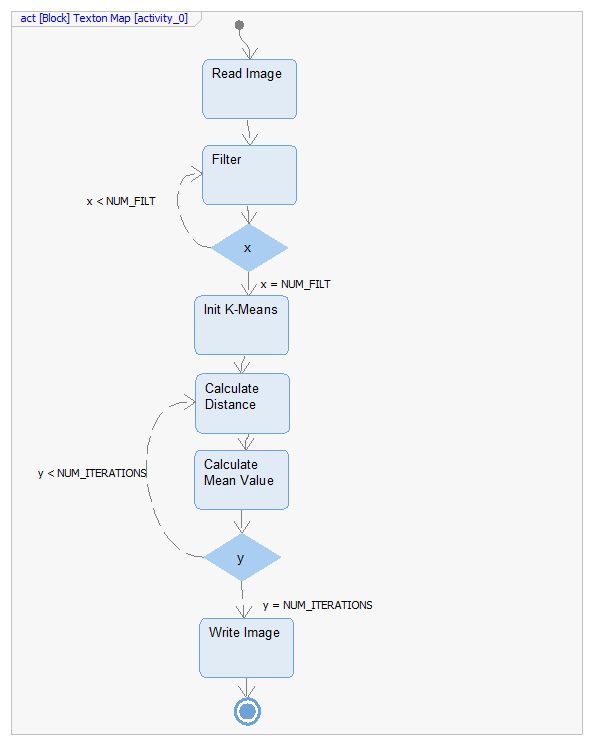
\includegraphics[width = 300 pt]{ActivityDiagram}
\caption{Activity diagram}
\label{fig:ActivityDiagram}
\end{figure}